\begin{center}
\begin{LARGE}
\title{Joanna Wojnowska}
\end{LARGE}
\end{center}
\section{Genetyka Kotów}

\subsection{Umaszczenie pręgowane}
\begin{flushleft}
Za obecność pręgowania na futrze odpowiada gen \textit{A – gen agouti}. Określa romieszczenie barwników, czarnej eumelaniny i rudej feomelaniny. Występuje w dwóch allelach \\
 \begin{center}
\textbf{allel A (agouti)} - dominujący\\
\textbf{allel a (non-agouti)} - recesywny
\end{center}
\begin{enumerate}
    
    \item \underline{Allel A} warunkuje występowanie umaszczenia pręgowanego. Pręgowanie jest efektem niejednolitego zabawienia pojedynczego kociego włosa. \item \underline{Allel A} powoduje naprzemienne zmniejszanie i zwiększanie wytwarzania barwnika, przez co na kocim włosie powstają jasne i ciemniejsze obszary.
    \item \underline{Allel A} nie powoduje powstawania prążków. Homozygotyczność powoduje, że eumelanina produkowana jest w nadmiarze, więc wypełnia włos na całej długości, powodując powstanie jednolitej barwy. Feomelanina przykryta zostaje eumelaniną przez co nie widać sferowego wybarwiania włosa. 
    \item \underline{Allel A} nie działa jednak na feomelaninę – jest ona nadal rozkładana strefowo, dlatego koty z genem rudności mają często widoczny wzór pręgowania. Stopień widoczności zależny jest od uwarunkowanej przez inne geny ilości produkowanego pigmentu. Koty rude i kremowe są bardzo często pręgowane pod względem fenotypowym, niezależnie od występowania u nich allelu recesywnego.
\end{enumerate}
\par
\begin{center}
\textbf{Kombinacje alleli:}
\end{center}

\begin{itemize}
\item[—] AA/Aa - kot pręgowany - zdjęcie \ref{fig:kot-pregowany} na stronie \pageref{fig:kot-pregowany}
\item[—] aa - kot jednolity - zdjęcie \ref{fig:kot-jednolity} na stronie \pageref{fig:kot-jednolity}
\end{itemize}
\clearpage

\subsection{Przykładowe zdjęcia}

\begin{figure}[h]
    \centering
    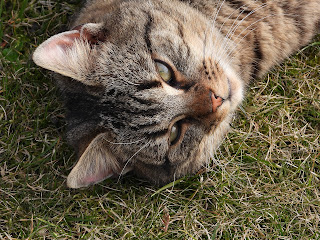
\includegraphics[width=0.5\textwidth]{pictures/kotpregowany.jpg}
    \caption{Kot pręgowany}
    \label{fig:kot-pregowany}
\end{figure}

\begin{figure}[h]
    \centering
    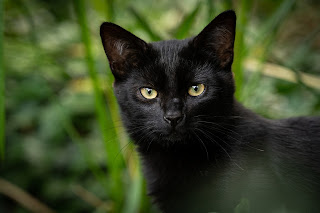
\includegraphics[width=0.5\textwidth]{pictures/kotjednolity.jpg}
    \caption{Kot jednolity}
    \label{fig:kot-jednolity}
\end{figure}


\subsection{Krzyżówki genetyczne}
Tabela \ref{tab:krzyzowka} zawiera przykładową krzyżówkę genetyczną dla potomstwa kota jednolitego i pręgowanego(będącego \underline{heterozygotą})

\begin{table}[htbp]
\centering
\begin{tabular}{c|c|c|}
\cline{2-3}
                                                         & \cellcolor[HTML]{C0C0C0}\textbf{A} & \cellcolor[HTML]{C0C0C0}\textbf{a} \\ \hline
\multicolumn{1}{|c|}{\cellcolor[HTML]{C0C0C0}\textbf{a}} & Aa                                 & aa                                 \\ \hline
\multicolumn{1}{|c|}{\cellcolor[HTML]{C0C0C0}\textbf{a}} & Aa                                 & aa                                 \\ \hline
\end{tabular}
\label{tab:krzyzowka}
\caption{Krzyżówka genetyczna: Aa x aa}
\end{table}


\subsection{Prawo Hardy’ego-Weinberga }
 Częstość alleli w populacji nie zmienia się z pokolenia na pokolenie
\[p^2 + q^2 +2pq =1\]
\[p + q = 1\]
\textit{p} – częstość występowania allelu A\\
\textit{q} – częstość występowania allelu a\\
$p^2$ – częstość występowania homozygoty dominującej (genotypu AA)\\
$q^2$– częstość występowania homozygoty recesywnej (genotypu aa)\\
$2pq$– częstość występowania heterozygoty Aa\\

Nowy tekst w overleafie\\
Kolejny nowy tekst w overleafie\\
Zmiany dokonane lokalnie\\
Więcej zmian dokonanych lokalnie
\end{flushleft}